\documentclass[a4,useAMS,usenatbib,usegraphicx,12pt]{article}
%External Packages and personalized macros
%=========================================================================
%		EXTERNAL PACKAGES
%=========================================================================
\usepackage[round]{natbib}
\usepackage[margin=3cm]{geometry}
\usepackage{hyperref}
\usepackage{times}
\usepackage{amsmath} 
\usepackage{amssymb}
\usepackage{graphicx}
\usepackage{array, xcolor, lipsum, bibentry}
\usepackage[nottoc, notlof, notlot]{tocbibind}

\definecolor{lightgray}{gray}{0.8}
\newcolumntype{L}{>{\raggedleft}p{0.14\textwidth}}
\newcolumntype{R}{p{0.8\textwidth}}
\newcommand\VRule{\color{lightgray}\vrule width 0.5pt}

\usepackage{booktabs}% http://ctan.org/pkg/booktabs
\newcommand{\tabitem}{~~\llap{\textbullet}~~}

%=========================================================================
%		INTERNAL MACROS
%=========================================================================
% To highlight comments 
\definecolor{red}{rgb}{1,0.0,0.0}
\newcommand{\red}{\color{red}}
\definecolor{darkgreen}{rgb}{0.0,0.5,0.0}
\newcommand{\SRK}[1]{\textcolor{darkgreen}{\bf SRK: \textit{#1}}}
\newcommand{\SRKED}[1]{\textcolor{darkgreen}{\bf #1}}

\newcommand{\LCDM}{$\Lambda$CDM~}
\newcommand{\beq}{\begin{eqnarray}}  
\newcommand{\eeq}{\end{eqnarray}}  
\newcommand{\zz}{$z\sim 3$} 
\newcommand{\apj}{ApJ}  
\newcommand{\apjs}{ApJS}  
\newcommand{\apjl}{ApJL}  
\newcommand{\aj}{AJ}  
\newcommand{\mnras}{MNRAS}  
\newcommand{\mnrassub}{MNRAS accepted}  
\newcommand{\aap}{A\&A}  
\newcommand{\aaps}{A\&AS}  
\newcommand{\araa}{ARA\&A}  
\newcommand{\nat}{Nature}  
\newcommand{\physrep}{PhR}
\newcommand{\pasp}{PASP}    
\newcommand{\pasj}{PASJ}    
\newcommand{\avg}[1]{\langle{#1}\rangle}  
\newcommand{\ly}{{\ifmmode{{\rm Ly}\alpha}\else{Ly$\alpha$}\fi}}
\newcommand{\hMpc}{{\ifmmode{h^{-1}{\rm Mpc}}\else{$h^{-1}$Mpc }\fi}}  
\newcommand{\hGpc}{{\ifmmode{h^{-1}{\rm Gpc}}\else{$h^{-1}$Gpc }\fi}}  
\newcommand{\hmpc}{{\ifmmode{h^{-1}{\rm Mpc}}\else{$h^{-1}$Mpc }\fi}}  
\newcommand{\hkpc}{{\ifmmode{h^{-1}{\rm kpc}}\else{$h^{-1}$kpc }\fi}}  
\newcommand{\hMsun}{{\ifmmode{h^{-1}{\rm {M_{\odot}}}}\else{$h^{-1}{\rm{M_{\odot}}}$}\fi}}  
\newcommand{\hmsun}{{\ifmmode{h^{-1}{\rm {M_{\odot}}}}\else{$h^{-1}{\rm{M_{\odot}}}$}\fi}}  
\newcommand{\Msun}{{\ifmmode{{\rm {M_{\odot}}}}\else{${\rm{M_{\odot}}}$}\fi}}  
\newcommand{\msun}{{\ifmmode{{\rm {M_{\odot}}}}\else{${\rm{M_{\odot}}}$}\fi}}  
\newcommand{\lya}{{Lyman$\alpha$~}}
\newcommand{\clara}{{\texttt{CLARA}}~}
\newcommand{\rand}{{\ifmmode{{\mathcal{R}}}\else{${\mathcal{R}}$ }\fi}}  


%MY COMMANDS #############################################################
\newcommand{\sub}[1]{\mbox{\scriptsize{#1}}}
\newcommand{\dtot}[2]{ \frac{ d #1 }{d #2} }
\newcommand{\dpar}[2]{ \frac{ \partial #1 }{\partial #2} }
\newcommand{\pr}[1]{ \left( #1 \right) }
\newcommand{\corc}[1]{ \left[ #1 \right] }
\newcommand{\lla}[1]{ \left\{ #1 \right\} }
\newcommand{\bds}[1]{\boldsymbol{ #1 }}
\newcommand{\oiint}{\displaystyle\bigcirc\!\!\!\!\!\!\!\!\int\!\!\!\!\!\int}
\newcommand{\mathsize}[2]{\mbox{\fontsize{#1}{#1}\selectfont $#2$}}
\newcommand{\eq}[2]{\begin{equation} \label{eq:#1} #2 \end{equation}}
\newcommand{\lth}{$\lambda_{th}$ }
%#########################################################################

\setlength\parindent{0pt}
 
\title{{\textbf{Research Proposal for a Master Thesis in Physics}}\\ 
				Verifying the VPH scheme in Galaxy Formation\\ 
				\color{black}\rule{15cm}{0.5mm}}
\author{Sebastian Bustamante Jaramillo}
\date{}
  
\begin{document}
\maketitle
\begin{center}
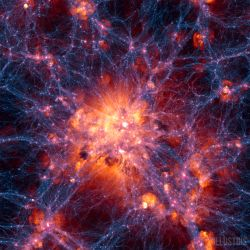
\includegraphics[trim = 0mm 3.5cm 0mm 3.0cm, clip, keepaspectratio=true,
width=0.7\textheight]{Presentation1.png}
\tiny{Time evolution of a gas cloud in a supersonic wind using a VPH scheme.
Taken from \citep{Hess10}}
\end{center}
\tableofcontents
 
\newpage 

%============================================================================== 
\section{General Information}
\small
\subsection*{Information of the Student}
\begin{tabular}{L!{\VRule}R}
\bf Name		& Sebastian Bustamante Jaramillo\\
\bf Degree		& B.Sc. in Physics, Universidad de Antioquia (2013)\\
\bf Position	& Adjunct Professor, Universidad de Antioquia\\
\bf Birthday	& { 20$^{th}$ June, 1990}\\
\bf Nationality & Colombian\\
\bf ID			& C.C. 1128400433\\
\bf Address 1	& Avenida 21 \# 57 AA 65, Bello - Colombia (personal)\\
\bf Address 2	& Calle 67 \# 53 - 108, Off. 5-330, Medellin, Colombia (work)\\
\bf Phone		& +057 (4) 4820138\\
\bf Mobile		& +057 3108992409\\
\bf E-mail 1	& macsebas33 \textit{at} gmail.com (personal)\\
\bf E-mail 2	& sebastian.bustamante \textit{at} udea.edu.co (academic)\\
\end{tabular}

\vspace{10pt}

More detailed information of the applicant can be found here \url{http://goo.gl/BPZGzK}

\vspace{15pt}  

\subsection*{Information of the Project}
\begin{tabular}{L!{\VRule}R}
\bf Title		& \bf Verifying the VPH scheme in Galaxy Formation\\
\bf Field		& Cosmology, Astrophysics, Physical Sciences \\
\bf Advisor 1	& Professor Juan Carlos Munoz-Cuartas. Universidad de Antioquia, Colombia.\\
\bf University	& Universidad de Antioquia, Master of Physics program \\
\bf Time Frame	& 2 years \\
\end{tabular}
\normalsize
%==============================================================================

%==============================================================================
\section{Abstract}
%==============================================================================
\newpage


%==============================================================================
\section{Introduction}
%==============================================================================


%==============================================================================
\section{Theoretical Framework}
%==============================================================================


%==============================================================================
\section{Objectives}
%==============================================================================


%==============================================================================
\section{Methodology}
%==============================================================================
\subsection*{General Objective}
\begin{itemize}
	\item Evaluating the performance of the \VPH method
\end{itemize}

%==============================================================================
\section{Expected Results}
%==============================================================================


%==============================================================================
\section{Scientific Impact}
%==============================================================================


%==============================================================================
\section{Schedule}
%==============================================================================


\begin{table}[h]
\begin{flushleft}
\begin{center}
  \begin{tabular}{l  l} \hline\hline
	\centering\textbf{Semester} & \textbf{Goals} \\ \hline
	%First year
	First  
	& \tabitem Identifying a set of existing \texttt{AREPO} simulations suitable 
	for our succeeding \\
	& \ \ \ \ studies. \\
	& \tabitem Applying web finding schemes (T-web and V-web) to the simulations 
	for\\
	& \ \ \ \ quantifying structures in the gaseous cosmic web, i.e. voids, walls, 
	filaments\\
	& \ \ \ \ and clusters.\\
	& \tabitem Evaluating properties of found structures at different redshifts.\\
	\\
	%Second year	
	Second
	& \tabitem Studying by mean of high resolution simulations the impact of the 
	gaseous\\
	& \ \ \ \ cosmic web on specific galaxy evolution processes.\\
	\\	
	
	\hline\hline
  \end{tabular}  
\end{center}
\end{flushleft}
\end{table}


%==============================================================================
\bibliographystyle{latex/mn2e}
\renewcommand{\bibname}{8\ \ \ \ Bibliography}
\small
\bibliography{references.bib}
%==============================================================================



\end{document}
